\documentclass{article}
\usepackage{amssymb}
\usepackage{amsmath}
\usepackage{indentfirst}
\usepackage{graphicx}
\usepackage{listings}
\usepackage{color}
\usepackage{float}
\definecolor{dkgreen}{rgb}{0,0.6,0}
\definecolor{gray}{rgb}{0.5,0.5,0.5}
\definecolor{mauve}{rgb}{0.58,0,0.82}

\lstset{frame=tb,
	language=Python,
	aboveskip=3mm,
	belowskip=3mm,
	showstringspaces=false,
	columns=flexible,
	basicstyle={\small\ttfamily},
	numbers=none,
	numberstyle=\tiny\color{gray},
	keywordstyle=\color{blue},
	commentstyle=\color{dkgreen},
	stringstyle=\color{mauve},
	breaklines=true,
	breakatwhitespace=true,
	tabsize=3
}

\author{Fu Min \ \ 72677006}
   \title{SI 211: Numerical Analysis\\ Homework 1 }
   
\begin{document}
\maketitle
\noindent \textbf{Problem 1}. We want to evaluate the function
	 \begin{align*}
	 	f(x) & = \frac{sin(10^{4}x)}{x}  	  
	 \end{align*}
\indent for different values of x.\\
\indent (a) Evaluate the above function at $ x = \pi$ by using Matlab, Julia, C++ or any other programming language of your choice. How big is the numerical approximation error? Can you explain why you observe this error?\\
\indent \textbf{Solution.}
   \begin{lstlisting}
      def problem1_f (x):
          F = sp.sin (10.0e4 * x)/x
          return F
      x1 = np.pi
      print ("F($\pi$)=",problem1_f(x1))
    \end{lstlisting}
    
      \indent  At  $x=\pi$, the exact solution is  f($\pi$)=0, while the solution by program is  $F(\pi)=-1.08100119082900e-11$. So the absolute rounding error is  $e=|f-F|=1.08100119082900e-11$. The order of magnitude the numerical approximation error is $10^{-11}$.\\ 
      \indent We get the derivative of $f(x)$ is 
      \begin{align*}
         f^{'}(x) = \frac{10^{4}*x*cos(10^{4}x)-sin(10^{4}x)}{x^2}
      \end{align*}
      \indent  At  $x=\pi$, the condition number is c = $f^{'}(\pi) = \frac{10^{4}}{\pi}$. So we can get that the order of magnitude the numerical approximation error is $10^{-11}$. \\
      
\indent (b)Evaluate the above function at $x = 10^{-10} $. How big is the numerical evaluation error?\\
%      \begin{lstlisting}
%         x2 = 10e-10
%         print ("F(10E-10)=", problem1_f(x2))
%      \end{lstlisting}
%  We can get that $F(10E-10)= 99999.9998333333$\\
   \indent  At  $x= 10^{-10}$, the condition number is c = $f^{'}(10^{-10})\approx 10^{14}$. So the numerical error is around
      \begin{align*}
      error & = c * eps\\
            & = f^{'}(10^{-10})* 2*10^{-16}\\
            & \approx 10^{-2}
      \end{align*}
\noindent \textbf{Problem 2}. Numeric differentiation based on central differences:\\
\indent (a) Implement a function (for example in Python, Julia, or Matlab) that uses numeric differentiation based on central differences,\\
  \begin{align*}
  	f^{'}(x) \approx\frac{f(x+h)-f(x-h)}{2h}
  \end{align*}
\indent Here, the inputs of the differentiation routine are the scalar function f that we want to differentiate, the point x at which the derivative should be evaluated, and the finite perturbation $h>0$. Use the syntax
   \begin{align*}
   \textbf{diff(f,x,h)} &= ...
   \end{align*}
   \textbf{Solution.}
   \begin{lstlisting}
   	  def diff(f,x,h):
   	      f_hat = (f(x + h) - f(x - h)) / (2.0 * h)
   	      error = np.abs(f_hat - f(x))
   	      return error
   \end{lstlisting}
   
\indent (b)Evaluate the derivative of the function $f(x) = exp(x)$ at $x = 0 $ using the above routine diff. Plot the numerical differentiation error in dependence on $ h  \in  [10^{-15},10^{-1}]$  and interpret the result. Use logarithmic scales on both axis!
\textbf{Solution.}\\
Code :
    \begin{lstlisting}
        f = np.exp
        x = 0.
        h = np.array([10.0**(-n) for n in range(1, 15)])
        error = diff(f,x,h)
        fig = plt.figure()
        axes = fig.add_subplot(1, 1, 1)
        axes.loglog(h, error, 's-', label="Centered")
        axes.legend(loc=3)
        axes.set_xlabel("h")
        axes.set_ylabel("Absolute Error")
        plt.show()
    \end{lstlisting}
The resulte:
  \begin{figure}[H]            \centering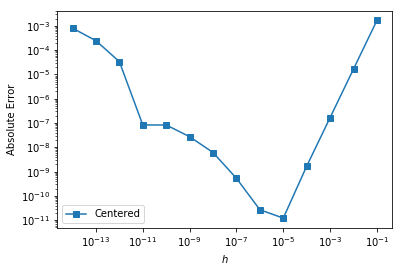
\includegraphics[width=2in,height=1.75in]{output_2.png}
	\caption{numerical differentiation error  VS  h}
	\label{fig:graph}
  \end{figure}


To the central differences, the mathematical approximation error is 

  

       $$\left| \frac{f(x+h)-f(x-h)}{2h}-\frac{\partial f}{\partial x}(x)\right| \leqslant \textbf{O}(h^{2}) $$

 The numerical error is still in the order of 

        $$ \frac{eps}{h} = \textbf{O}(\frac{eps}{h}) $$

 At $x=0$, the condition number is c = $f^{'}(0)=1$. So the $f$ is well conditioned. We can choose $h \approx \sqrt[3]{eps}\approx 10^{-5}$. It still verifies the minmun in figure 1.

\noindent \textbf{problem 3.} In order to evaluate the factorable function $f (x) = sin(cos(x))\ast cos(x)^{2}$ we write an evaluation algorithm of the form
    \begin{align*}
    a_{0} &= x\\
    a_{1} &= cos(x)\\
    a_{2} &= a_{1} \ast a_{1}\\
    a_{3} &= sin(a_1)\\
    a_{4} &= a_{2} \ast a_{3}\\
    f(x)  & = a_{4}
    \end{align*}
\indent  What is the corresponding algorithm for evaluating the derivative of $f(x)$ using the forward mode of algorithmic differentiation (AD)? What is the order of magnitude of the numerical error that is associated with evaluating the derivative of $f$ at $x = 0$ using this AD code?\\
\textbf{Solution.}\\
The AD is:
      \begin{align*}
         b_{0} &= 1\\
         b_{1} &= -six(x)\\
         b_{2} &= b_{1} \ast a_{1}+ a_{1}*b_{1}\\
         b_{3} &= cos(a_1) \ast  b_{1} \\
         b_{4} &= b_{2} \ast a_{3} + a_{2} \ast b_{3} \\
         f^{'}(x)  & =b_{4}
      \end{align*}
The code :
     \begin{lstlisting}
         def AD(x):
           a0 = x
           a1 = sp.cos(x)
           a2 = a1 * a1
           a3 = sp.sin(a1)
           a4 = a2 * a3
           b0 = 1
           b1 = -1* sp.sin(x)
           b2 = b1 * a1 + a1 *b1
           b3 = sp.cos(a1) * b1 
           b4 = b2 * a3 + a2*b3
           return a4, b4
         f, diff_f = AD(0.)
     \end{lstlisting}
 From the above program, we can get that $f^{'}(0) = 0$. So the order of magnitude of the numerical error is 0.
\end{document} 